\documentclass{article}

\PassOptionsToPackage{numbers}{natbib}
\usepackage[final]{nips_2018}

\usepackage[utf8]{inputenc} % allow utf-8 input
\usepackage[T1]{fontenc}    % use 8-bit T1 fonts
\usepackage{hyperref}       % hyperlinks
\usepackage{url}            % simple URL typesetting
\usepackage{booktabs}       % professional-quality tables
\usepackage{amsfonts}       % blackboard math symbols
\usepackage{nicefrac}       % compact symbols for 1/2, etc.
\usepackage{microtype}      % microtypography
\usepackage{graphicx}
\usepackage{float}
\bibliographystyle{plainnat}

\newcommand{\quotes}[1]{``#1''}

\title{\quotes{Attention Is All You Need} Digested}

\author{
  Sepehr Sameni\\
  Department of Artificial Intelligence\\
  University of Tehran\\
  \texttt{sepehr.sameni@gmail.com} \\
}

\begin{document}

\maketitle

\begin{abstract}
  In this short document, I will discuss the strengths and weaknesses of \quotes{Attention is all you need}\citep{1706.03762} by looking at the follow-up papers and conclude with some potential improvements on top of transformers based on high computational complexity.
\end{abstract}

\section{Sequence to Sequence Models}
One of the most powerful formulations of many machine learning problems is seq2seq. Given an input sequence, we seek to generate the corresponding output sequence with a possibly different length than the input. Although this is a vague definition, It used to be implemented as a recurrent encoder followed by a recurrent decoder\citep{1409.3215}. This vanilla solution has four major problems:

\begin{enumerate}
  \item long training time caused by the sequential nature of the encoder and decoder.
  \item long inference time caused by the autoregressive decoder.
  \item order dependency in encoder and decoder, even though it’s not a problem for text and we can almost always read and write words from left to right(this has also been challenged recently by \citep{1808.07910}), it is not clear how to best read pixels of a picture\citep{1712.09763}
  \item the information bottleneck; encoding the whole sequence into one fixed size vector is not efficient and posses hard restrictions on the encoder.
\end{enumerate}

There has been a lot of research to solve these problems including: \citep{1409.0473} that introduced an attention mechanism in the decoder and solved the information bottleneck(we should note that the tradeoff here is that they also increased the memory consumption of the network during inference), convolutional encoder and decoder\citep{1705.03122} that addressed the first issue by introducing a non recurrent building block for encoding and decoding, the tradeoff here is the depth, in order for the network to be able to model long dependencies of the input, they had to increase the depth of the network.

The next step toward improving seq2seq is using something without order dependence in the encoder which Transformers achieve pretty well and interestingly enough they obtain better results with shorter training times.

It is also important to note that even though this paper is mainly focused on NMT, seq2seq has many more applications, including image caption generation\citep{1411.4555}, video captioning\citep{1505.00487}, Speech recognition\citep{1712.01769}, speech generation\citep{1609.03499}, language modeling\citep{1810.04805}, document classification\citep{1707.00896} and even multi task learning\citep{1706.05137}.

\section{Transformer}
In this paper, authors ditched rnn and cnn altogether and replaced them with only self-attention and cross attention, by doing this they were able to achieve state of the art results on NMT with a fraction of computing power compared to the previous state of the art results.
In the following sections, I will talk about different components of their model, talk about their pros and cons and cite papers about those individual parts.

\subsection{Attention}
Bahdanau et al\citep{1409.0473} introduced attention to decoders and since then we have seen a lot of improvements caused by attention\citep{1611.04558} and it makes sense to assume that it is a crucial part of modern NMT and using it in the encoder(which is a novel thing in this paper) should yield higher accuracy(BLEU score). Although this is a sensible assumption, it does not have any mathematical proofs supporting it and might be wrong altogether as challenged in You May Not Need Attention\citep{1810.13409}

Another reason in favor of using attention is the more explainability of the network that for years had been assumed to be true. Even though by using multi-head attention they have weakened this point, explainability is still possible in transformer networks\citep{1809.03985}. But this assumption can be wrong, in the recently published paper titled Attention is not Explanation\citep{1902.10186} authors show that attention weights are not necessary interpretable.

The silver bullet is that attention mechanism helps the vanishing gradient by reducing the maximum dependency length between tokens and that is enough to explain their training efficiency. But are they here to stay? Do we have any mathematical proofs for their expressibility? First, in the paper called Universal Transformers\citep{1807.03819} authors show that under mild assumptions, Recurrent Transformers can be Turing Complete and it might mean that RNNs can be replaced with their Transformer counterpart.

Another interesting line of research is to prove that Transformers (or a variant of them) are Universal function approximators like \citep{1804.10306} that shows any translation equivariant function can be approximated arbitrarily well by a convolutional neural network given that it is sufficiently wide, in direct analogy to the classical universal approximation theorem.

One of the missing things in the paper is that they talked about restricted attention and compared them with other models in the first table but there are no experiments on them. I know that implementing them efficiently is really hard (and maybe impossible given the current memory layouts) but they could implement them via attention masking and compare the results to show whether full sequence attention in the base model is leveraged or not.(see figure \ref{fig:rattention})

\begin{figure}[H]
  \centering
  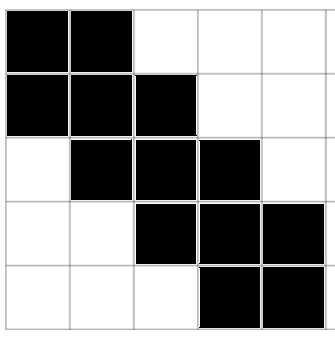
\includegraphics[scale=0.20]{restricted.png}
  \caption{Resctricted Attenttion Map with $n=5$ and $r=3$}
  \label{fig:rattention}
\end{figure}

Another missing experiment for the Attention module is the lack of self-attention visualization in the decoder, it makes sense for the encoder to learn meaningful attention weights (like coreference resolution and parsing) but what does the decoder’s masked self-attention show? Is it a masked version of the same things? Or something non-interpretable for humans?. Also, attention visualization in figure 5 is not that informative and the caption of the figure is rather vague.

\subsection{Multi-Head Attention}
Explanation of multi-head attention is pretty clear, and it’s a great way to combat the lower resolution precision that comes with attention averaging and there is an ablation study on the number of heads but they didn’t visualize how increasing or decreasing the number of heads can hurt the network’s performance.

Implicitly different heads learn different concepts and that is interesting but the tradeoff here is that it increases the possibility of overfitting and probably increasing the training time. One can easily combat this with another implicit method like Weighted Transformers\citep{1711.02132} by introducing a few trainable parameters and encouraging difference between heads. It is also shown in\citep{1810.10183}, applying a disagreement regularizer to explicitly encourage different heads to attend to different locations helps to overcome overfitting and it even helps to encode our prior knowledge about the sentence in heads\citep{1804.08199}

\subsection{Layer-Norm}
The paper does not explain the necessity of layer norm in training and the intuition on choosing layer norm instead of the batch norm(we know that layer norm is better than the batch norm when we have recurrent modules but what about transformers?)

Another general issue with normalization layers is their lack on understanding, as it is shown recently in\citep{1805.11604} common belief about batch norm, that they control the change of the layers’ input distributions during training to reduce the so-called “internal covariate shift” does not hold true and indeed it makes the loss landscape more smooth. But we don’t have such a theory for layer norm and using it is just practical but not mathematically sound. On top of these, it has recently been shown\citep{1901.09321} that with careful initialization we can drop batch norm and layer norm layers and train even deeper networks without any issues and obtain better results than the base transformer in NMT.

\subsection{Position Embedding}
The necessity of position embedding is clear but it is not clear how the addition of them to the word vectors changes the behavior of word vectors and helps the network to understand the position.
They also justified their choice of position embedding based on sine and cosine with dependence on only starting position vector and distance(but not the other position vector) but they didn’t do any experiments on this and didn’t show that the network is capable of generating and consuming sequences longer than the ones seen during training.

As future studies show, position embedding is much more important and explicitly modeling the relative distance can improve the results\citep{1803.02155} and improved in \citep{1901.02860} by including an inductive bias raised from the sinusoid encoding matrix.

\subsection{Feed Forward Network}
It is not clear how the FFN helps the training and why it is needed, it can be argued that they are inserted to make the whole network nonlinear but it is not true because attention is not linear and even though the output of the network, if we only used self-attention layers, is just a linear combination of all tokens but it is input dependent and thus nonlinear. Once again this shows that we need a better theoretical understanding of Transformers in order to justify the FFN. Another point worth mentioning is that it seems FFN play an important role in the Transformer because they are not replaced in The Evolved Transformer\citep{1901.11117}.

\subsection{Masked Decoder}
Decoding is inherently sequential and forcing our network to work sequentially via masking is a bit unnatural and it forces the decoder to work in a strange way, as I said replacing calculated self-attention with uniform averaging does not decrease accuracy and it means that we can do better, as it is stated in \citep{1804.09849}: ''On  the  other  hand,  lacking  a  memory component (as present in the RNN models) prevents  the  network  from  modeling  a  state  space,reducing  its  theoretical  strength  as  a  sequence model, ...'' they showed that combining a self-attentive encoder and a recurrent decoder improves accuracy (with the cost of increased training time) and I think it’s a reasonable middle ground.

\subsection{Inference}
Even though it’s not part of this paper’s goals but it worth mentioning that autoregressive models like this will not improve the inference time and as a matter of fact it will increase the memory budget for inference because of the self-attention in decoder that needs to store all intermediate presentations for previous tokens for the current token which can be solved with an embarrassingly simple idea like \citep{1805.00631} which is surprising, it seems that self-attention in the decoder is not that important and once again it raises the question that what does the self-attention in decoder learns and bothers the reader with this lack of experiment.

Another interesting idea to improve inference time is to use a Non-Autoregressive NMT by replacing the teacher forcing method of training with token fertilities and using the full power of decoder(no masked attention) to generate the whole output sequence in one pass and reduce the latency by an order of magnitude\citep{1711.02281}

\subsection{Experiments}
The ablation study is good and it aligns well with the paper claims and authors’ intuitions. But I would love it if there were a multilingual translation study to show that the self-attention mechanism can be language independent. It was perfect if they also showed something like CoVE\citep{1708.00107} and show the power of the leaned encoder as a contextualized word embedding extractor.
The constituency parsing is not well explained and they are just there to make the paper a bit longer, I think there are many better applications for seq2seq that could have been shown to impress the reader. But overall the experiments are sound and they are well developed.

\section{Possible Improvements}
\subsection{Capsule Attention}
\subsubsection{Problem Statement}
The computational complexity of transformer networks are quadratic in sequence length($\mathcal{O}(n^{2}d)$) and that prevents them to be used on mobile devices or large audio sequences

\subsubsection{Possible Solution}
I argue that the full attention is not necessary for the network and it suffices for the network to only attend to the most important concepts of the sequence. So instead of generating a $K$(key) and $V$(value) with size $n$ for the attention, we can generate them with much lower size $k$(which can be a constant number like 16) via an EM algorithm like \citep{1805.10807} or even vanilla soft K-means over the full $K$ and $V$.
So as in the base transformer, we calculate $K$, $V$, and $Q$ then instead of calculating the dot product between $K$ and $Q$ we first summarize $K$ from size $n*d$ to $k*d$ via weight-less dynamic routing and we use the same weights to also summarize the $V$ into $k*d$, afterward we calculate attention between $Q$ and the summarized $K$ and multiply by the summarized $V$ which yields a sequence of size $n*d$ as before but with a much lower computational complexity of $\mathcal{O}(nkd)$

\subsubsection{Prevoius Work}
As shown in Star Transformer\citep{1902.09113}, we can propagate information into different nodes with a single intermediate node, which is like setting $k$ in CAT to $1$, but one should note that Start Transformer is applied for $T$ times in each layer and those calculations are dependent and cannot be parallelized, in contrast in CAT all $k$ centers are calculated in parallel and there are no iterations(except for the kmeans which can take as little as 2 iterations)

Another similar work is\citep{1811.00287} which uses capsule networks at the last step of encoder but CAT is the extreme case of that idea and applies this idea in all the layers of both encoder and decoder's self-attention

\citep{1812.01243} also tried to make attention linear in sequence length by changing the order of attention calculation and come up with an $\mathcal{O}(nd^{2})$ algorithm which is more compute expensive than CAT for typical network sizes.

As shown in \citep{1901.11117} and \citep{1901.10430} convolution is still relevant and combining convolution networks for local relation extraction and CAT for global context extraction seems legit.

\subsubsection{Possible Application}
Not only we might be able to train larger BERT\citep{1810.04805} or GPT-2 models and improve the current state of the art NLP models.
With such an algorithm we can easily apply self-attention to much longer inputs like pixels and audio and improve GAN results\citep{1805.08318}.
In theory, we should be able to use CAT in all seq2seq tasks and improve their results by training larger models and better-representing context.

\subsection{Dilated Attention}
\subsubsection{Problem Statement}
The computational complexity of transformer networks are linear in depth($\mathcal{O}(ln^{2}d)$) and that prevents them to be used on mobile devices or large audio sequences.

\subsubsection{Possible Solution}
We can use self-attention dilation to reduce their complexity to $\mathcal{O}(2n^{2}d) = \mathcal{O}(n^{2}d)$ by using exponentially grown dilation rate in upper layers of the network as shown in figure \ref{fig:dattention}. Once again I argue that at least with the current methods, full-sequence attention is not being utilized and most transformer networks are under fitted and this is great opportunity to weaken their structure and fully utilize the resulting network.

\begin{figure}[H]
  \centering
  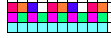
\includegraphics[]{dilated.png}
  \caption{Dilated Self Attention(nodes with the same color are analyzed together)}
  \label{fig:dattention}
\end{figure}

\subsubsection{Prevoius Work}
Time\citep{1803.01271} and time again\citep{1710.02224} it has been shown that dilation improves parameter efficiency and final accuracy of the networks.

\subsection{Mobile Transformer}
\subsubsection{Problem Statement}
As I mentioned multi-head attention is overparameterized and it can be easily regularized either via implicit methods over explicit ones.

\subsubsection{Possible Solution}
I want to implement a regularizer by architecture design that resembles separable convolutions\citep{1704.04861} and light convolutions\citep{1901.10430}. Instead of having different heads that use different projection weights we first split the input and project resulting parts and at the end instead of using another linear layer on the concatenated vector, I rely on the FFN to fuse inputs (like mobile net's 1x1 cnn)

\subsubsection{Calculations}
for the vanilla transformer model we have $3(key, value, query) * h(heads) * d_{model}(input) * d_{qkv}(intermediate) + h(concat) * d_{qkv}(intermediate) * d_{model}(final) + d_{model}(ffn_{input}) * d_{ff}(intermediate) + d_{ff} * d_{model}(final)$ which is 3145728 for the base model.
for the mobile version(with a moved residual connection) we have $3 * h * d_{model} // h(splited) * d_{qkv} + 0$(no need to resize intermediate representation)$+ h * d_{qkv} * d_{ff} + d_{ff} * d_{model}$ which is equal to 2195456, one million parameters saved per layer for 12 layers of encoder and decoder in base-transformer we can reduce the total parameters by 20\%

\bibliography{citations}

\end{document}
